\documentclass[notheorems,serif,table,compress]{beamer}  %dvipdfm选项是关键,否则编译统统通不过
%%------------------------常用宏包------------------------
%%注意, beamer 会默认使用下列宏包: amsthm, graphicx, hyperref, color, xcolor, 等等
\usepackage{fontspec,xunicode,xltxtra}  % for XeTeX
\usepackage{verbatim}
\usepackage{mathabx}
\usepackage{latexsym}
\usepackage{amsfonts,amssymb}
\usepackage{styles/iplouclistings}
\usepackage{fancybox}
\usepackage{colortbl}
\usepackage{tcolorbox}
%\usepackage[T1]{fontenc}
%\usepackage{bookman}
\usepackage{subfigure}
\usepackage{hyperref}
\usepackage{listings}
\usepackage{animate}
\usepackage[absolute,overlay]{textpos}
\usepackage{graphicx}
\usepackage{tikz}
\usepackage[americaninductors,europeanresistors]{circuitikz}
\usepackage{tikz}
\usepackage{fancybox}     %% 定义zhushadow时用到
\usepackage{pifont} %ding用到
\newsavebox{\mysaveboxOne}  %%为了在only中使用lstlisting
\newsavebox{\mysaveboxTwo}
\newsavebox{\mysaveboxThree}
\newsavebox{\mysaveboxFour}
\newsavebox{\mysaveboxFive}
\newsavebox{\mysaveboxSix}
\newsavebox{\mysaveboxSeven}
\newcommand\zhushadow[2][purple]{\hskip5pt\shadowbox{\color{#1}\small\kai #2\vspace{3mm}}}

%%------------------------ThemeColorFont------------------------
%% Presentation Themes
% \usetheme[<options>]{<name list>}
%\usetheme{Madrid}
\usetheme{Berkeley}
%% Inner Themes双精度计算
% \useinnertheme[<options>]{<name>}
%% Outer Themes
% \useoutertheme[<options>]{<name>}
%\useoutertheme{miniframes} 
%% Color Themes 
%\usecolortheme[<options>]{<name list>}
%% Font Themes
\usefonttheme{serif}
\setbeamertemplate{background canvas}[vertical shading][bottom=white,top=structure.fg!7] %%背景色, 上25%的蓝, 过渡到下白.
\setbeamertemplate{theorems}[numbered]
\setbeamertemplate{navigation symbols}{}   %% 去掉页面下方默认的导航条.
\usepackage{styles/zhfontcfg}
%\setsansfont[Mapping=tex-text]{文泉驿正黑}  %% 需要fontspec宏包
     %如果装了Adobe Acrobat,可在font.conf中配置Adobe字体的路径以使用其中文字体
     %也可直接使用系统中的中文字体如SimSun,SimHei,微软雅黑 等
     %原来beamer用的字体是sans family;注意Mapping的大小写,不能写错
     %设置字体时也可以直接用字体名,以下三种方式等同:
     %\setromanfont[BoldFont={黑体}]{宋体}
     %\setromanfont[BoldFont={SimHei}]{SimSun}
     %\setromanfont[BoldFont={"[simhei.ttf]"}]{"[simsun.ttc]"}
%%------------------------MISC------------------------
\graphicspath{{figures/}}         %% 图片路径. 本文的图片都放在这个文件夹里了.
%%------------------------listing------------------------
%\lstset{language=[LaTeX]TeX,Python}
%%------------------------正文------------------------
\begin{document}
\XeTeXlinebreaklocale "zh"         % 表示用中文的断行
\XeTeXlinebreakskip = 0pt plus 1pt % 多一点调整的空间
%%----------------------------------------------------------
%% This is only inserted into the PDF information catalog. Can be left
%% out.
%%%
%% Delete this, if you do not want the table of contents to pop up at
%% the beginning of each subsection:
%\AtBeginSection[]{                              % 在每个Section前都会加入的Frame
%  \frame<handout:0>{
%    \frametitle{Contents}\small
%    \tableofcontents[current,currentsubsection]
%  }
%}
%
%\AtBeginSubsection[]                            % 在每个子段落之前
%{
%  \frame<handout:0>                             % handout:0 表示只在手稿中出现
%  {
%    \frametitle{Contents}\small
%    \tableofcontents[current,currentsubsection] % 显示在目录中加亮的当前章节
%  }
%}

\setbeamertemplate{caption}{\raggedright\insertcaption\par}

%%----------------------------------------------------------
\logo{
\includegraphics[scale=0.13]{ouclogo.png}}
\title{Cluster-based Segmentation }
\subtitle{基于聚类的图像分割}
\author[]{\textcolor{olive}{WangRuchen}}
\institute[CVBIOUC]
{
\small\textcolor{violet}{CVBIOUC\\
%Ocean University of China\\
\url{http://vision.ouc.edu.cn/~zhenghaiyong}}
}
%\date[]{}
%\titlegraphic{
%
\includegraphics[height=1.0cm]{ouc-logo.jpg}}
\frame{ \titlepage }
%%----------------------------------------------------------
%\section*{Contents}
\frame{\frametitle{Contents}\tableofcontents}
%%----------------------------------------------------------
\def\hilite<#1>{\temporal<#1>{\color{blue!15}}{\color{black}}{\color{black}}}
\newcommand{\shadow}[2][purple]{\hskip5pt\shadowbox{\color{#1}\small \kai #2\vspace{3mm}}}
\newcommand{\colorrbox}[2][purple]{\doublebox{\color{#1}\small \kai#2}}

%============================================================================

\section{Introduction}

%============================================================================

\subsection{Clustering Analysis}
\begin{frame}[fragile]
\frametitle{Clustering Analysis}
    ~~~~Clustering is {\color{blue}unsupervised classification}: no predefined classes.\newline
    
{\color{blue}Cluster:} a collection of data objects
    \begin{itemize}
      \item Similar to one another within the same cluster 
      \item Dissimilar to the objects in other clusters
    \end{itemize}
\end{frame}

\subsection{Image Segmentation with Clustering}
\begin{frame}
\frametitle{Image Segmentation with Clustering}
{\color{blue}Idea:}

Cluster similar pixel features together.\newline

{\color{blue}How to segment images by clustering?}
    \begin{figure}
      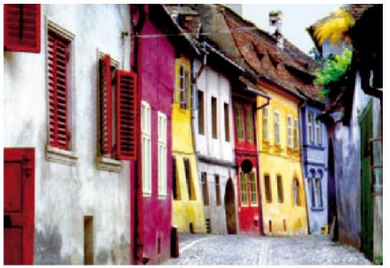
\includegraphics[width=0.6\linewidth]{clustering1.png}
    \end{figure}
\end{frame}

\begin{frame}
\frametitle{Image Segmentation with Clustering}
   \centering \qquad \quad Image \quad $\Longrightarrow$ \quad Feature space\newline

\pause
{\color{blue}Feature space:}(R,G,B),(R,G,B,X,Y),(L,U,V)$\cdots$
    \begin{figure}
      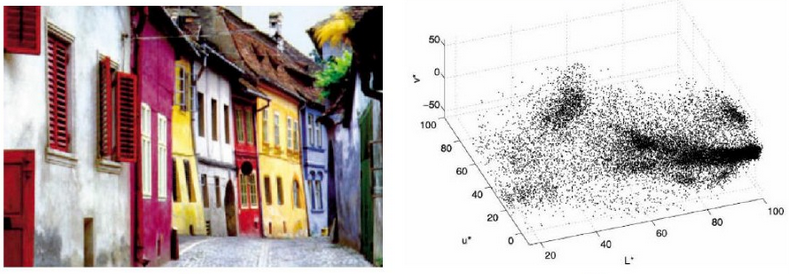
\includegraphics[width=0.8\linewidth]{clustering.png}
    \end{figure}
\end{frame}
 
 \begin{frame}
\frametitle{Image Segmentation with Clustering}
    \begin{columns}
        \begin{column}{0.5\linewidth}
          \begin{itemize}
          \item Vector Clustering
          \end{itemize}
          \begin{figure}
          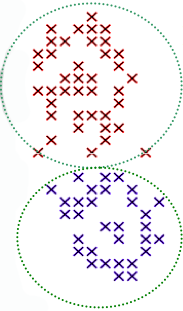
\includegraphics[width=0.3\linewidth]{vc.png} 
          \end{figure}
          Each point has a vector.
        \end{column}
        \begin{column}{0.45\linewidth}
          \begin{itemize}
          \item Graph Clustering
          \end{itemize}
          \begin{figure}
          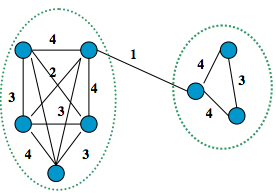
\includegraphics[width=0.7\linewidth]{gc.png} 
          \end{figure}
          Each vertex is connected to others by edges.
        \end{column}
    \end{columns}\vspace{1ex}
\end{frame}
 
 \begin{frame}
\frametitle{Image Segmentation with Clustering}
   \centering \qquad \quad Image \quad $\Longrightarrow$ \quad Feature space\newline

{\color{blue}Feature space:}(R,G,B),(R,G,B,X,Y),(L,U,V)$\cdots$
    \begin{figure}
      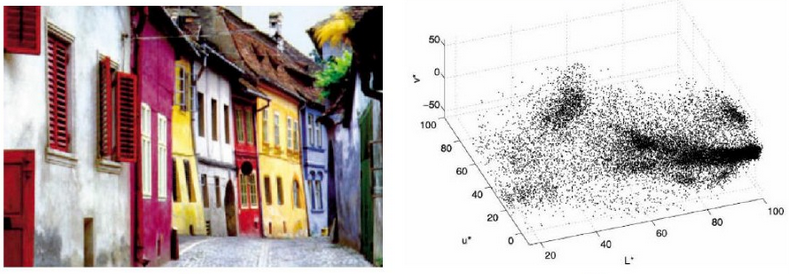
\includegraphics[width=0.8\linewidth]{clustering.png}
    \end{figure}
\end{frame}
 
\begin{frame}
\frametitle{Image Segmentation with Clustering}
{\color{blue}Techniques}:
    \begin{itemize}
      \item K-means
      \item Mean Shift
    \end{itemize}
\end{frame}

%============================================================================

\section{K-means}

%============================================================================



\subsection{Idea}
\begin{frame}
\frametitle{K-means}
{\color{blue}Idea:}
    \begin{enumerate}
      \item Randomly initialize the K cluster centers.
      \item For each point, find the closest cluster centers. Put the point into the cluster. 
      \item Change the cluster centers.
    \end{enumerate}
    \begin{figure}
      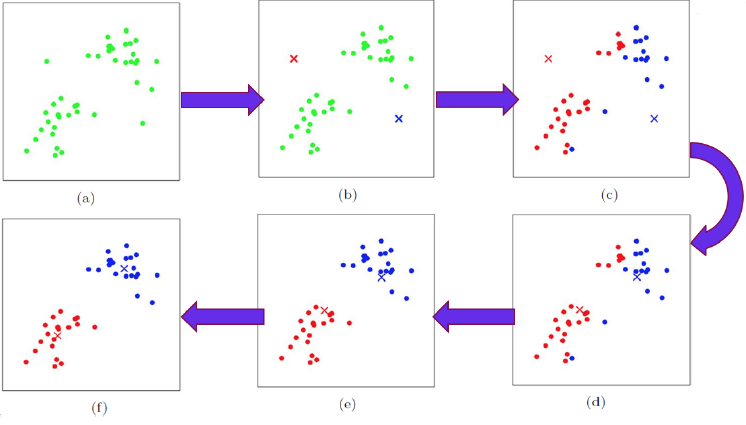
\includegraphics[width=0.7\linewidth]{kmean1.png} 
    \end{figure}
\end{frame}

\subsection{Algorithm}
\begin{frame}
\frametitle{K-means}
    {\color{blue}Algorithm:}
    \begin{enumerate}
      \item Choose randomly K-means $m_{1},\dots, m_{k}$.
      \item For each vector $x_{i}$ compute $D(x_{i},m_{k}(ic)), k=1,\dots,K$ and assign $x_{i}$ to the cluster $C_{j}$ with nearest mean.
      \item Update the means to get $m_{1}(ic),\dots,m_{K}(ic)$.
          \begin{displaymath}
            m_{i}^{(t+1)}=\frac{1}{|S_{i}^{(t)}|}\sum_{x_{j}\in S_{i}^{(t)}}x_{j}
          \end{displaymath}
      \item Repeat steps 2 and 3 until $C_{k}(ic) = C_{k}(ic+1)$ for all k.
    \end{enumerate}
\end{frame}

\subsection{}
\begin{frame}
\frametitle{K-means}
{\color{blue}Pros:}
    \begin{itemize}
      \item Simple and fast
      \item Converges to a local minimum of the error function
    \end{itemize}
{\color{blue}Cons:}
    \begin{itemize}
    \item {\color{blue}Sensitive to initialization}
    \item Need to pick K
    \end{itemize}
\end{frame}

\subsection{K-means++}
\begin{frame}
\frametitle{K-means++\footnote{Arthur, D. and Vassilvitskii, S, ``K-means++: The Advantages of Careful Seeding'', PA, 2007.}}
{\color{blue}Algorithm:}
    \begin{enumerate}
      \item Take one center $c_{1}$, chosen uniformly at random from $X$.
      \item Take a new center $c_{i}$, choosing $x \in X$ with probability $\frac{D(x)^{2}}{\sum_{x \in X}D(x)^{2}}$.
      \item Repeat Step2, until we have taken $k$ centers altogether.
      \item Proceed as with the standard K-means algorithm.\newline
      
    \end{enumerate}
    ~~~~$D(x)$ denote the shortest distance from a data point to the closest center we have already chosen.
\end{frame}

\begin{frame}
\frametitle{K-means}
{\color{blue}Pros:}
    \begin{itemize}
      \item Simple and fast
      \item Converges to a local minimum of the error function
    \end{itemize}
{\color{blue}Cons:}
    \begin{itemize}
    \item Sensitive to initialization 
    \item {\color{blue}Need to pick K}
    \end{itemize}
\end{frame}

%============================================================================

\section{Mean Shift}

%============================================================================

\begin{frame}
\frametitle{Mean Shift\footnote{D. Comaniciu and P. Meer, ``Mean Shift: A Robust Approach toward Feature Space Analysis'', PAMI, 2002. }}
~~~~An advanced and versatile technique for clustering-based segmentation.\newline

{\color{blue}Idea:}
    \begin{itemize}
    \item Find the {\color{blue}clustering center}. 
    \end{itemize}
    \begin{figure}
      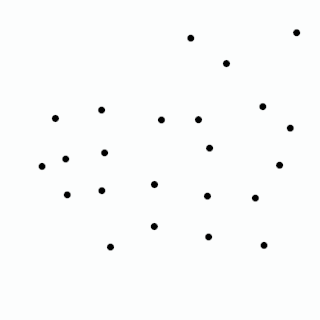
\includegraphics[width=0.25\linewidth]{julei.png} 
    \end{figure}
\end{frame}

\subsection{Idea}
\begin{frame}
\frametitle{What and How?}
    \begin{figure}
      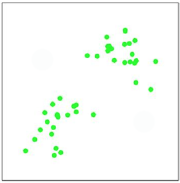
\includegraphics[width=0.25\linewidth]{zhong.png} 
    \end{figure}
    \pause
Center is maximum points of probability density function and gradient direction.\newline
\end{frame}

\begin{frame}
\frametitle{Mean Shift Vector}
    \begin{figure}
    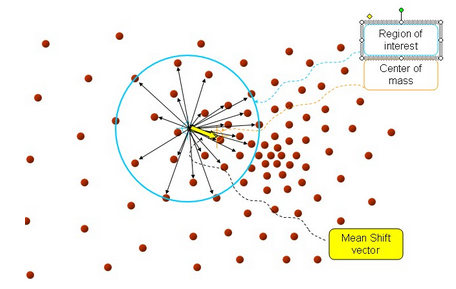
\includegraphics[width=0.5\linewidth]{msv.png}
    \end{figure}
    \begin{displaymath}
    M_{h}=\frac{1}{K}\sum_{x_{i}S_{k}}(x_{i}-x)
    \end{displaymath}
\end{frame}

\subsection{What is Mean Shift}
\begin{frame}
\frametitle{What is Mean Shift}
    \begin{figure}
      \begin{minipage}[t]{0.45\linewidth}
      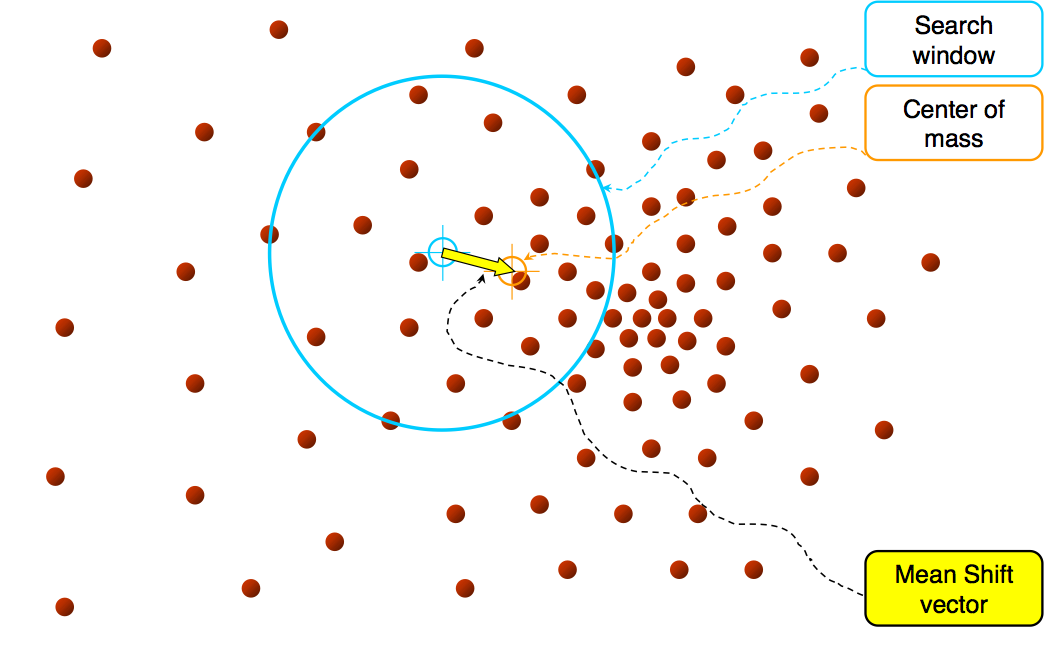
\includegraphics[width=1\linewidth]{meanshift1.png} 
      \end{minipage}
      \pause
      \begin{minipage}[t]{0.45\linewidth}
      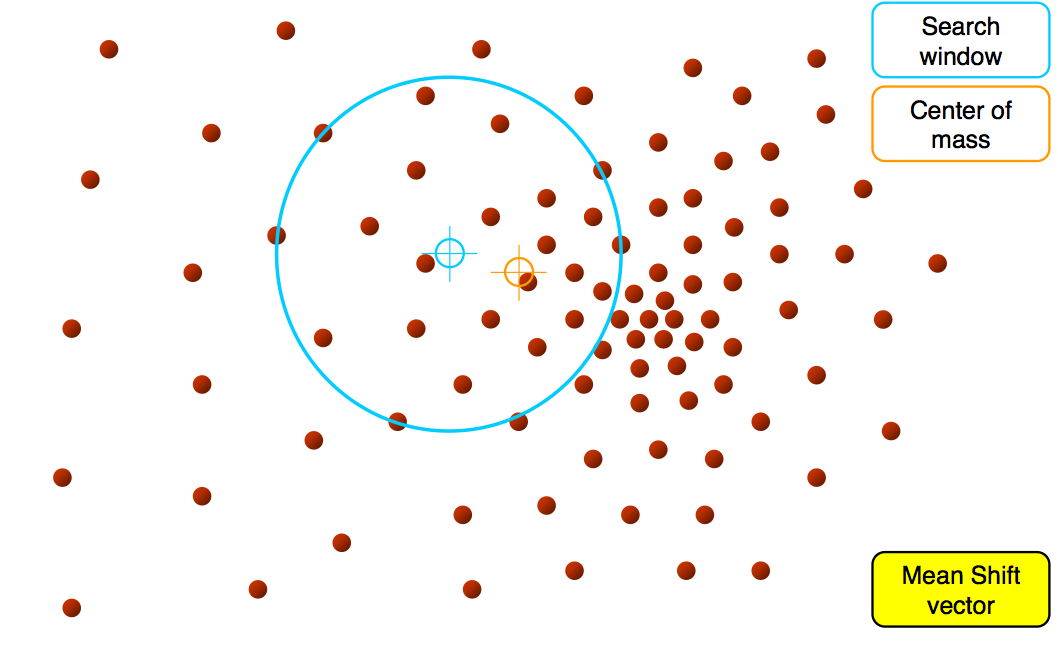
\includegraphics[width=1\linewidth]{meanshift2.png} 
      \end{minipage}
    \end{figure}
    \pause
    \begin{figure}
      \begin{minipage}[t]{0.45\linewidth}
      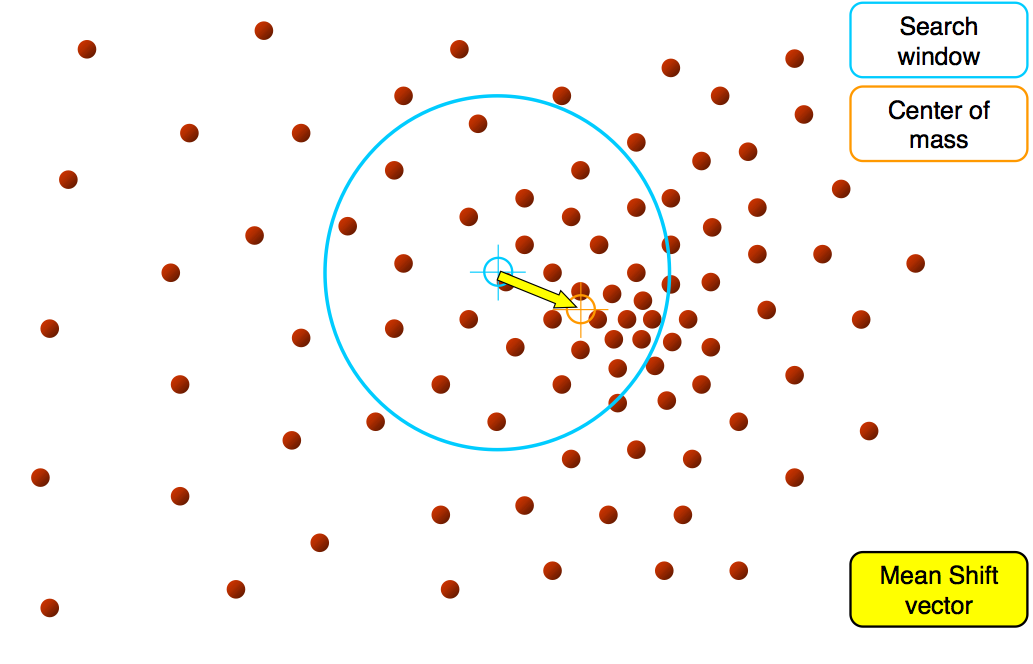
\includegraphics[width=1\linewidth]{meanshift3.png} 
      \end{minipage}
      \pause
      \begin{minipage}[t]{0.45\linewidth}
      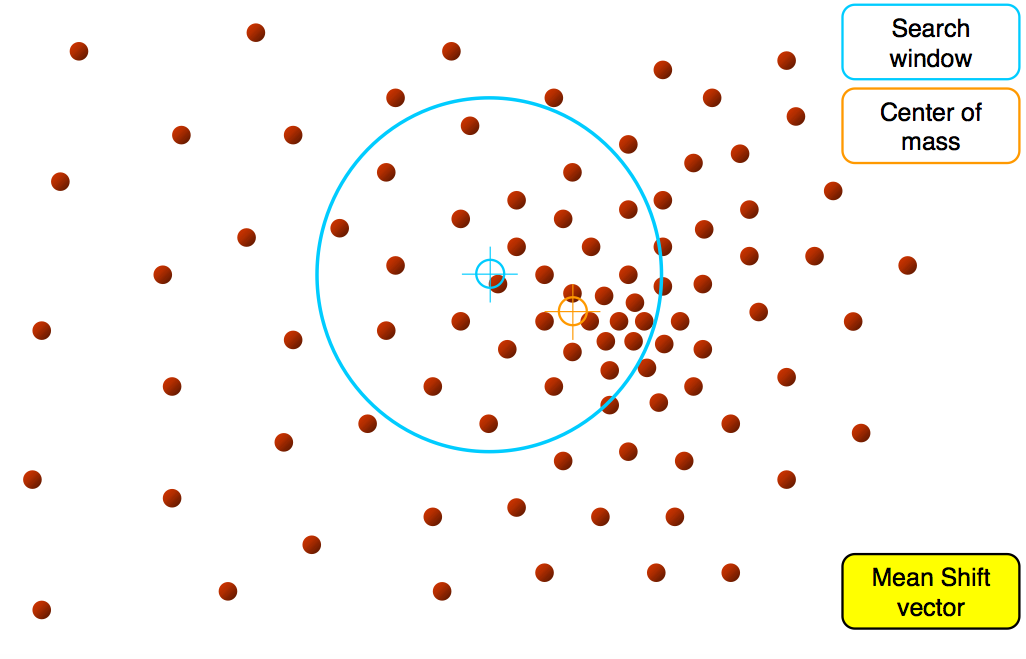
\includegraphics[width=1\linewidth]{meanshift4.png} 
      \end{minipage}
    \end{figure}
\end{frame}

\begin{frame}
\frametitle{What is Mean Shift}
    \begin{figure}
      \begin{minipage}[t]{0.45\linewidth}
      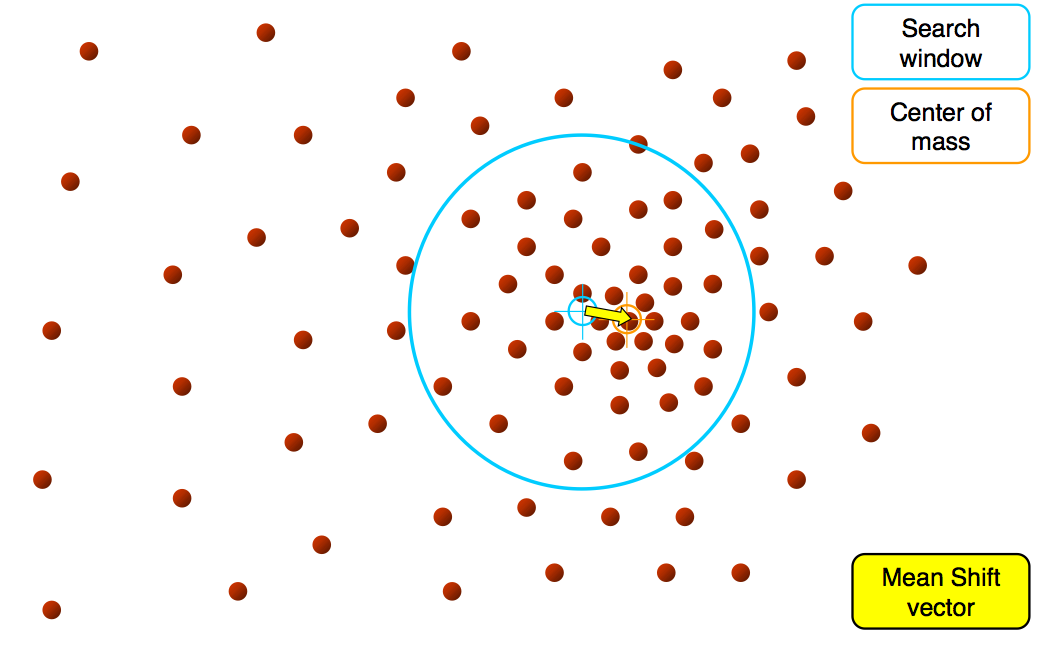
\includegraphics[width=1\linewidth]{meanshift5.png} 
      \end{minipage}
      \pause
      \begin{minipage}[t]{0.45\linewidth}
      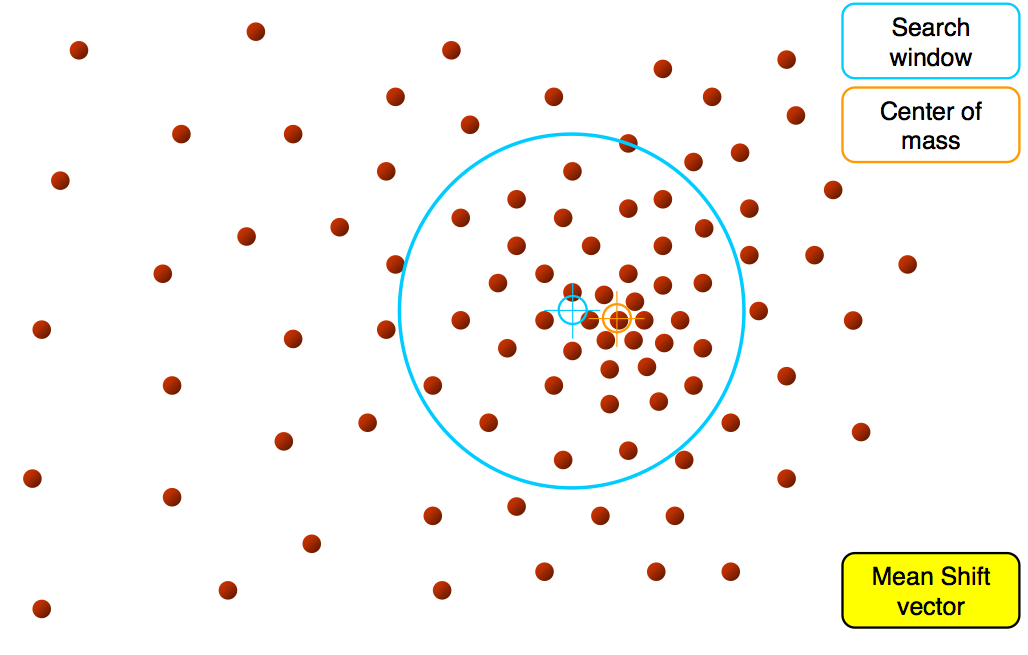
\includegraphics[width=1\linewidth]{meanshift6.png} 
      \end{minipage}
    \end{figure}
    \pause
    \begin{figure}
      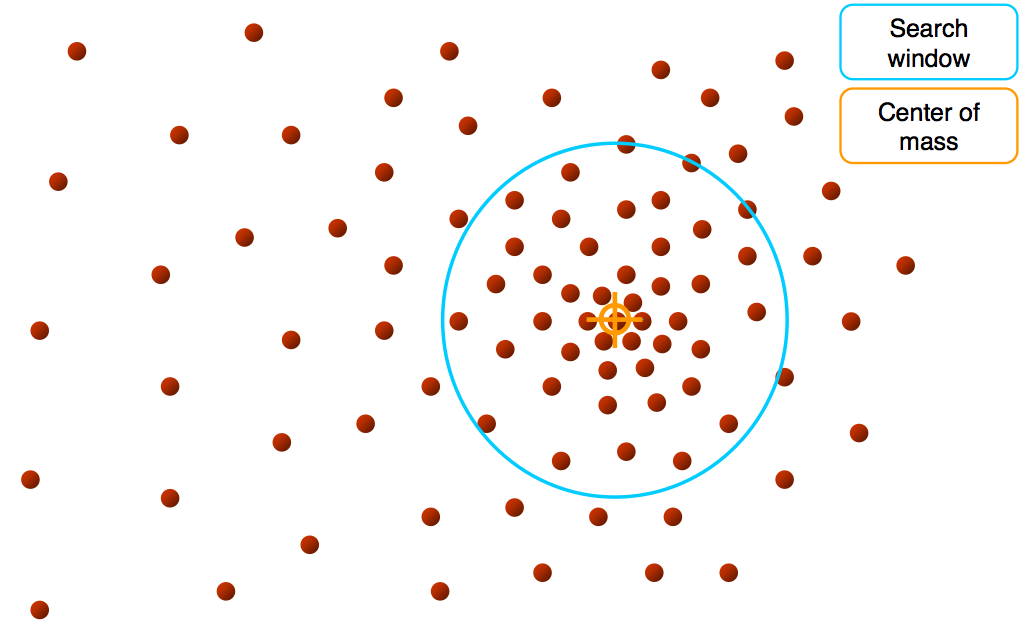
\includegraphics[width=0.45\linewidth]{meanshift7.png} 
    \end{figure}
\end{frame}

\begin{frame}
\frametitle{What is Mean Shift}
    \begin{figure}
      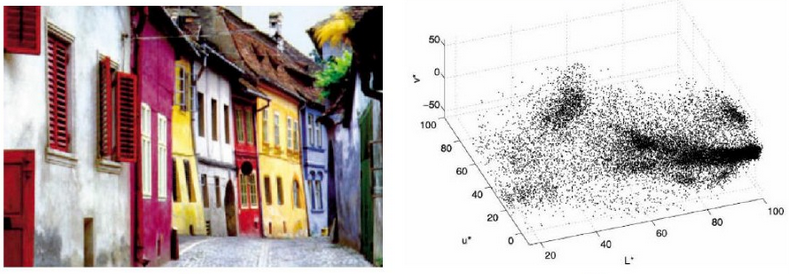
\includegraphics[width=0.8\linewidth]{clustering.png} 
    \end{figure}
\end{frame}

\subsection{Why}
\begin{frame}
\frametitle{Density Estimation}
    \begin{figure}
      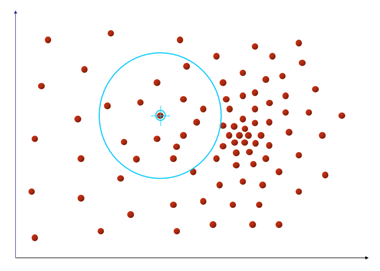
\includegraphics[width=0.45\linewidth]{midu.png} 
    \end{figure}
    \begin{displaymath}
            P=\frac{N_{k}}{N}
     \end{displaymath}
     \begin{displaymath}
            f(x)=\frac{P}{S}=\frac{N_{k}}{NS}
      \end{displaymath}
\end{frame}

\begin{frame}
\frametitle{Kernel density estimation (Parzen windows)}
{\color{blue}Kernel density estimation:}

~~~~Let $(x_{1}, x_{2}, …, x_{n})$ be an independent and identically distributed sample drawn from some distribution with an unknown density $f(x)$. Its kernel density estimator is
\begin{columns}
        \begin{column}{0.55\linewidth}
          \begin{flalign*}
           \hat{f(x)_{h,k}}=\frac{1}{Nh^{d}}\sum_{n=1}^{N}k(\frac{x_{n}-x}{h})
           \end{flalign*}
    Kernel function:
          \begin{displaymath}
            k(u)= \left\{  \begin{array}{ll}
                  1 & |u_{i}| \le \frac{1}{2}, i=1,\dots, D\\
                  0 & otherwise\\
                  \end{array} \right.
          \end{displaymath}
         \end{column}
         \begin{column}{0.45\linewidth}
          \begin{figure}
           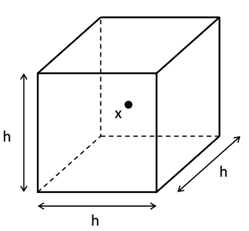
\includegraphics[width=0.6\linewidth]{hemidu.png} 
          \end{figure}
          \end{column}
    \end{columns}\vspace{1ex}
\end{frame}

\begin{frame}
\frametitle{Kernel density estimation}
          \begin{displaymath}
            \hat{f}_{h,K}(x)=\frac{1}{Nh^{d}}\sum_{n=1}^{N}k(||\frac{x-x_{n}}{h}||^{2})
           \end{displaymath}
Density gradient:
          \begin{displaymath}
            \hat{\bigtriangledown}f_{h,K}(x)=\frac{2}{Nh^{d+2}}\sum_{n=1}^{N}(x_{n}-x)[-k'(||\frac{x-x_{n}}{h}||^{2})]
          \end{displaymath}
          \begin{displaymath}
            g(x)=-k'(x)
          \end{displaymath}
\end{frame}

\begin{frame}
\frametitle{Kernel density estimation}
          \begin{flalign*}
            \hat{\bigtriangledown}&f_{h,K}(x)=\frac{2}{Nh^{d+2}}\sum_{n=1}^{N}(x_{n}-x)[g(||\frac{x-x_{n}}{h}||^{2})]&\\
                  &  =\underbrace{\frac{2}{h^{2}}}_{C}\underbrace{[\frac{1}{Nh^{d}}\sum_{n=1}^{N}g(||\frac{x_{n}-x}{h}||^{2})]}_{\hat{f_{h,G}(x)}}\underbrace{[\frac{\sum_{n=1}^{N}x_{n}g(||\frac{x_{n}-x}{h}||^{2})}{\sum_{n=1}^{N}g(||\frac{x_{n}-x}{h}||^{2})}-x]}_{m_{h,G}(x)}&\\
          \end{flalign*}
\end{frame}

\begin{frame}
\frametitle{Kernel density estimation}
    \begin{figure}
    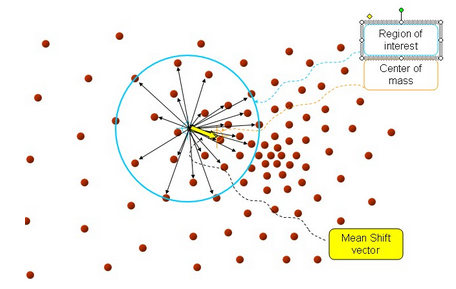
\includegraphics[width=0.5\linewidth]{msv.png}
    \end{figure}
    \begin{displaymath}
    M_{h}=\frac{1}{K}\sum_{x_{i}S_{k}}(x_{i}-x)
    \end{displaymath}
\end{frame}

\begin{frame}
\frametitle{Kernel density estimation}
\begin{columns}
        \begin{column}{0.55\linewidth}
          \begin{displaymath}
            m_{h,G}(x)=\frac{\sum_{n=1}^{N}x_{n}g(||\frac{x_{n}-x}{h}||^{2})}{\sum_{n=1}^{N}g(||\frac{x_{n}-x}{h}||^{2})}-x
          \end{displaymath}
          \begin{displaymath}
          m_{h,G}(x)=0
          \end{displaymath}
        \end{column}
        \begin{column}{0.45\linewidth}
         \begin{figure}
         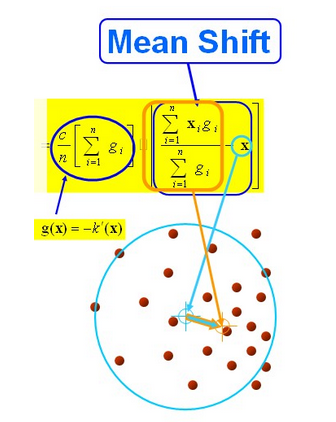
\includegraphics[width=0.8\linewidth]{tu.png} 
         \end{figure}
        \end{column}
    \end{columns}\vspace{1ex}
\end{frame}

\begin{frame}
\frametitle{Kernel density estimation}
    \begin{figure}
      \begin{minipage}[t]{0.45\linewidth}
      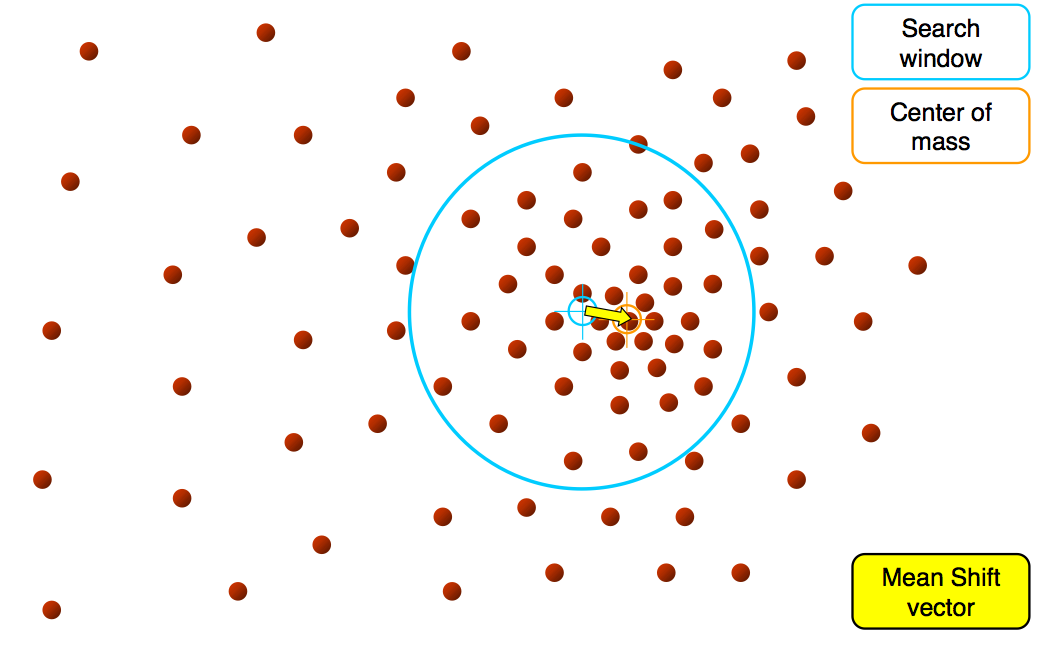
\includegraphics[width=1\linewidth]{meanshift5.png} 
      \end{minipage}
      \begin{minipage}[t]{0.45\linewidth}
      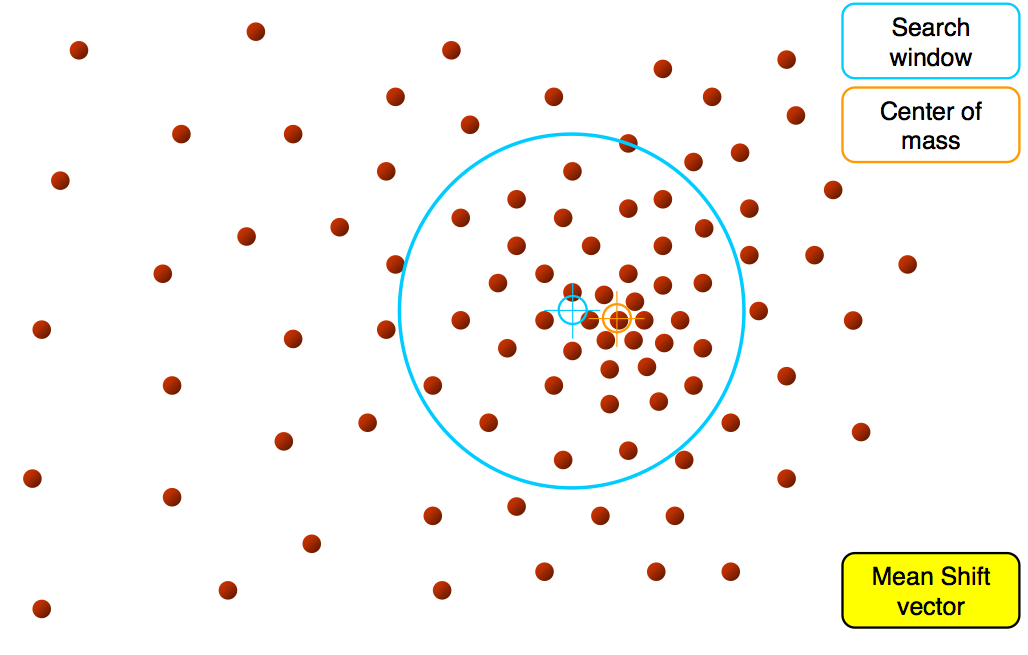
\includegraphics[width=1\linewidth]{meanshift6.png} 
      \end{minipage}
    \end{figure}
    \begin{figure}
      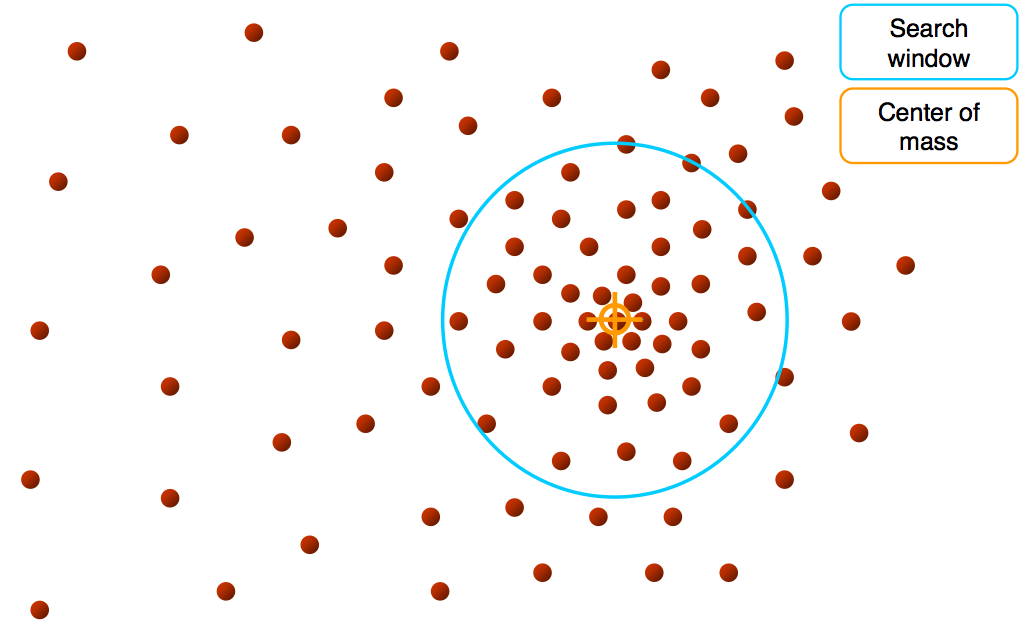
\includegraphics[width=0.45\linewidth]{meanshift7.png} 
    \end{figure}
\end{frame}


\begin{frame}
\frametitle{Kernel density estimation}

Clustering center:
          \begin{displaymath}
              y_{i,k+1}=\frac{\sum_{n=1}^{N}x_{n}g(||\frac{x_{n}-x}{h}||^{2})}{\sum_{n=1}^{N}g(||\frac{x_{n}-x}{h}||^{2})}
           \end{displaymath}
\end{frame}

\subsection{Algorithm}
\begin{frame}
\frametitle{Mean Shift}
    {\color{blue}Algorithm:}
    \begin{enumerate}
      \item Find features(color, gradients, texture, etc).
      \item Initialize windows at individual pixel locations.
      \item Compute $y_{i,k+1}$ until convergence, $y_{i,k}=y_{i,k+1}$.
      \item Assign $z_{i}=(x_{i},y_{i,k})$.
    \end{enumerate}
\end{frame}

\begin{comment}
\begin{frame}
\frametitle{Mean Shift}
{\color{blue}Pros:}
    \begin{itemize}
      \item Just a single paramete(window size)
      \item Finds variable number of modes
      \item Robust to outliers
    \end{itemize}
{\color{blue}Cons:}
    \begin{itemize}
    \item Output depends on window size
    \item Computationally expensive
    \end{itemize}
\end{frame}
\end{comment}

\begin{frame}
  \vspace{2cm}
  \centering
  \color{blue}\Huge{Thanks!}
  \vspace{1.5cm}
 

\end{frame}
%===============================================================================


\end{document}
